\documentclass{IEEEtran}
\usepackage[spanish]{babel}
\usepackage[utf8]{inputenc}
\usepackage{enumerate}
\usepackage{cite}
\usepackage{graphicx} 
\usepackage{float} 
\usepackage{subfig}

\hyphenation{op-tical net-works semi-conduc-tor}


\begin{document}
\title{Paralelización Efecto de Desenfoque}
\author{\IEEEauthorblockN{Carlos Arturo Romero Lopez, Bryan Antonio Angarita Rodriguez\\}
\IEEEauthorblockA{Universidad Nacional Bogotá, Colombia \\
Email:caralopezrom@unal.edu.co, baangaritar@unal.edu.co\\}
}
\maketitle

\begin{abstract}
Operar bajo el principio de que una tarea se puede dividir en tareas más pequeñas y ejecutarlo de forma simultanea permite optimizar, por lo menos en tiempo y consumo de recursos, la ejecución de procesos.
\\

Existen herramientas que facilitan o dificultan en cierto grado esta tarea, por ejemplo, \textit{POSIX} es una API que permite trabajar con hilos a muy bajo nivel, esto implica mayor control sobre la creación uso destrucción de los mismos, mientras que por otro lado, Open MP (OMP) es una herramienta de alto nivel que es portable y facil de usar y escalar.
\end{abstract}

\section{Introducción}

El siguiente documento se muestra el uso de paralelización en un algoritmo para el desenfoque de una imagen, en el proceso se usarán varías herramientas para mostrar las ventajas y desventajas que puedan tener cada una de ellas, por ejemplo, se implementará el algoritmo de forma secuencia, así mismo se usarán las herramientas de paralelización POSIX Threads (Pthreads) y Open MP (OMP) variando el numero de hilos a utilizar y el numero de Kernel (distancia en el algoritmo) para así observar en tiempo cual puede llegar a ser más eficiente.


\subsection{Efecto de desenfoque.}
Para el desarrollo de esta practica se hará uso de la librería opencv para procesamiento de imagenes y del algoritmo de deseonfoque gaussiano.

\subsubsection{Desenfoque gaussiano}
El algoritmo de desenfoque gaussiano consiste básicamente en el que cada pixel de la imagen tendrá como valor el promedio de todos los valores de los pixeles vecinos en un radio definido.

Esto se puede ver de la siguiente forma, sea b(i, j) nuestra matriz con desenfoque gaussiano
\\
\begin{equation}
\centering
•b[i, j] = \sum\limits_{y = i - r}^{i + r} \sum\limits_{x = j - r}^{j + r} f[y, x] * w[y, x]
\end{equation}
\\
Donde r sería el radio a cubrir, es decir, el kernel del desenfoque.

\begin{figure}[htb]
\centering
\includegraphics[height=1in]{bRN2c}
\caption{Desenfoque gaussiano.} \label{fig:fig1}
\end{figure}

\section{Paralelización del algoritmo.}

Lo primero que se efectua dentro del programa es la verificación de los parametros, pues es necesario que se defina previamente el numero de hilos y el tamaño del kernel a usar, despues de eso se hace uso de la librería opencv para generar una copia de la imagen, inmediatamente  verificados los parametros se procede a la creación de una estructura de tipo datoHilo que la que tendrá en escencia la información a cerca de el objetivo del hilo especifico y luego sí se crean los hilos como dependiendo del modelo que vayamos a evaluar \textit{Secuencial, POSIX, OMP}, para la creación de hilos se hará uso de  \textit{pthread\_create} y \textit{\#pragma omp parallel} para POSIX y OMP respectivamente.
\\

Respecto a cómo se dividió la imagen para el proceso de paralelización; en el procedimiento segmento() se asigna acada uno de las estructuras datoHilo, creadas previamente en una matriz, el identificador del hilo y punto de inicio y final tanto en $x$ como en $y$ dentro de la imagen así, el identificador se asigna de forma secuencial dentro de una estructura for y el segmento de la imagen que vaya a trabajar cada hilo esto es, se divide, el numero de filas y columnas de la imagen original en partes iguales segun el número de hilos y el tamaño del radio (kernel) que se haya definido previamente.


\section{Experimentos y resultados.}
El algoritmos implementado en C con la libreria opencv y bajo las formas de paralelización OMP y POSIX se probaron así:

\begin{enumerate}
\item Se varió el numero de hilos con un tamaño de kernel constante, en este casó se uso un kernel de 9 obteniendo los siguientes valores\\
\begin{table}[H]
\centering
\begin{tabular}{|p{1.5cm}||p{1.5cm}|p{1.5cm}|p{1.5cm}| }
\hline 
•&	720p&	1080p&	4k \\
\hline 
\hline 
1&	0.79&	3.77&	14.98 \\
3&	0.34&	1.60&	6.56 \\
5&	0.32&	1.37&	5.78 \\
7&	0.30&	1.39&	5.94 \\
9&	0.30&	1.37&	6.06 \\
11&	0.29&	1.37&	6.15 \\
13&	0.29&	1.40&	6.08 \\	
\hline		
\end{tabular} 
\caption{Tiempos con POSIX} \label{table:table1}
\end{table}
\begin{figure}[H]
\centering
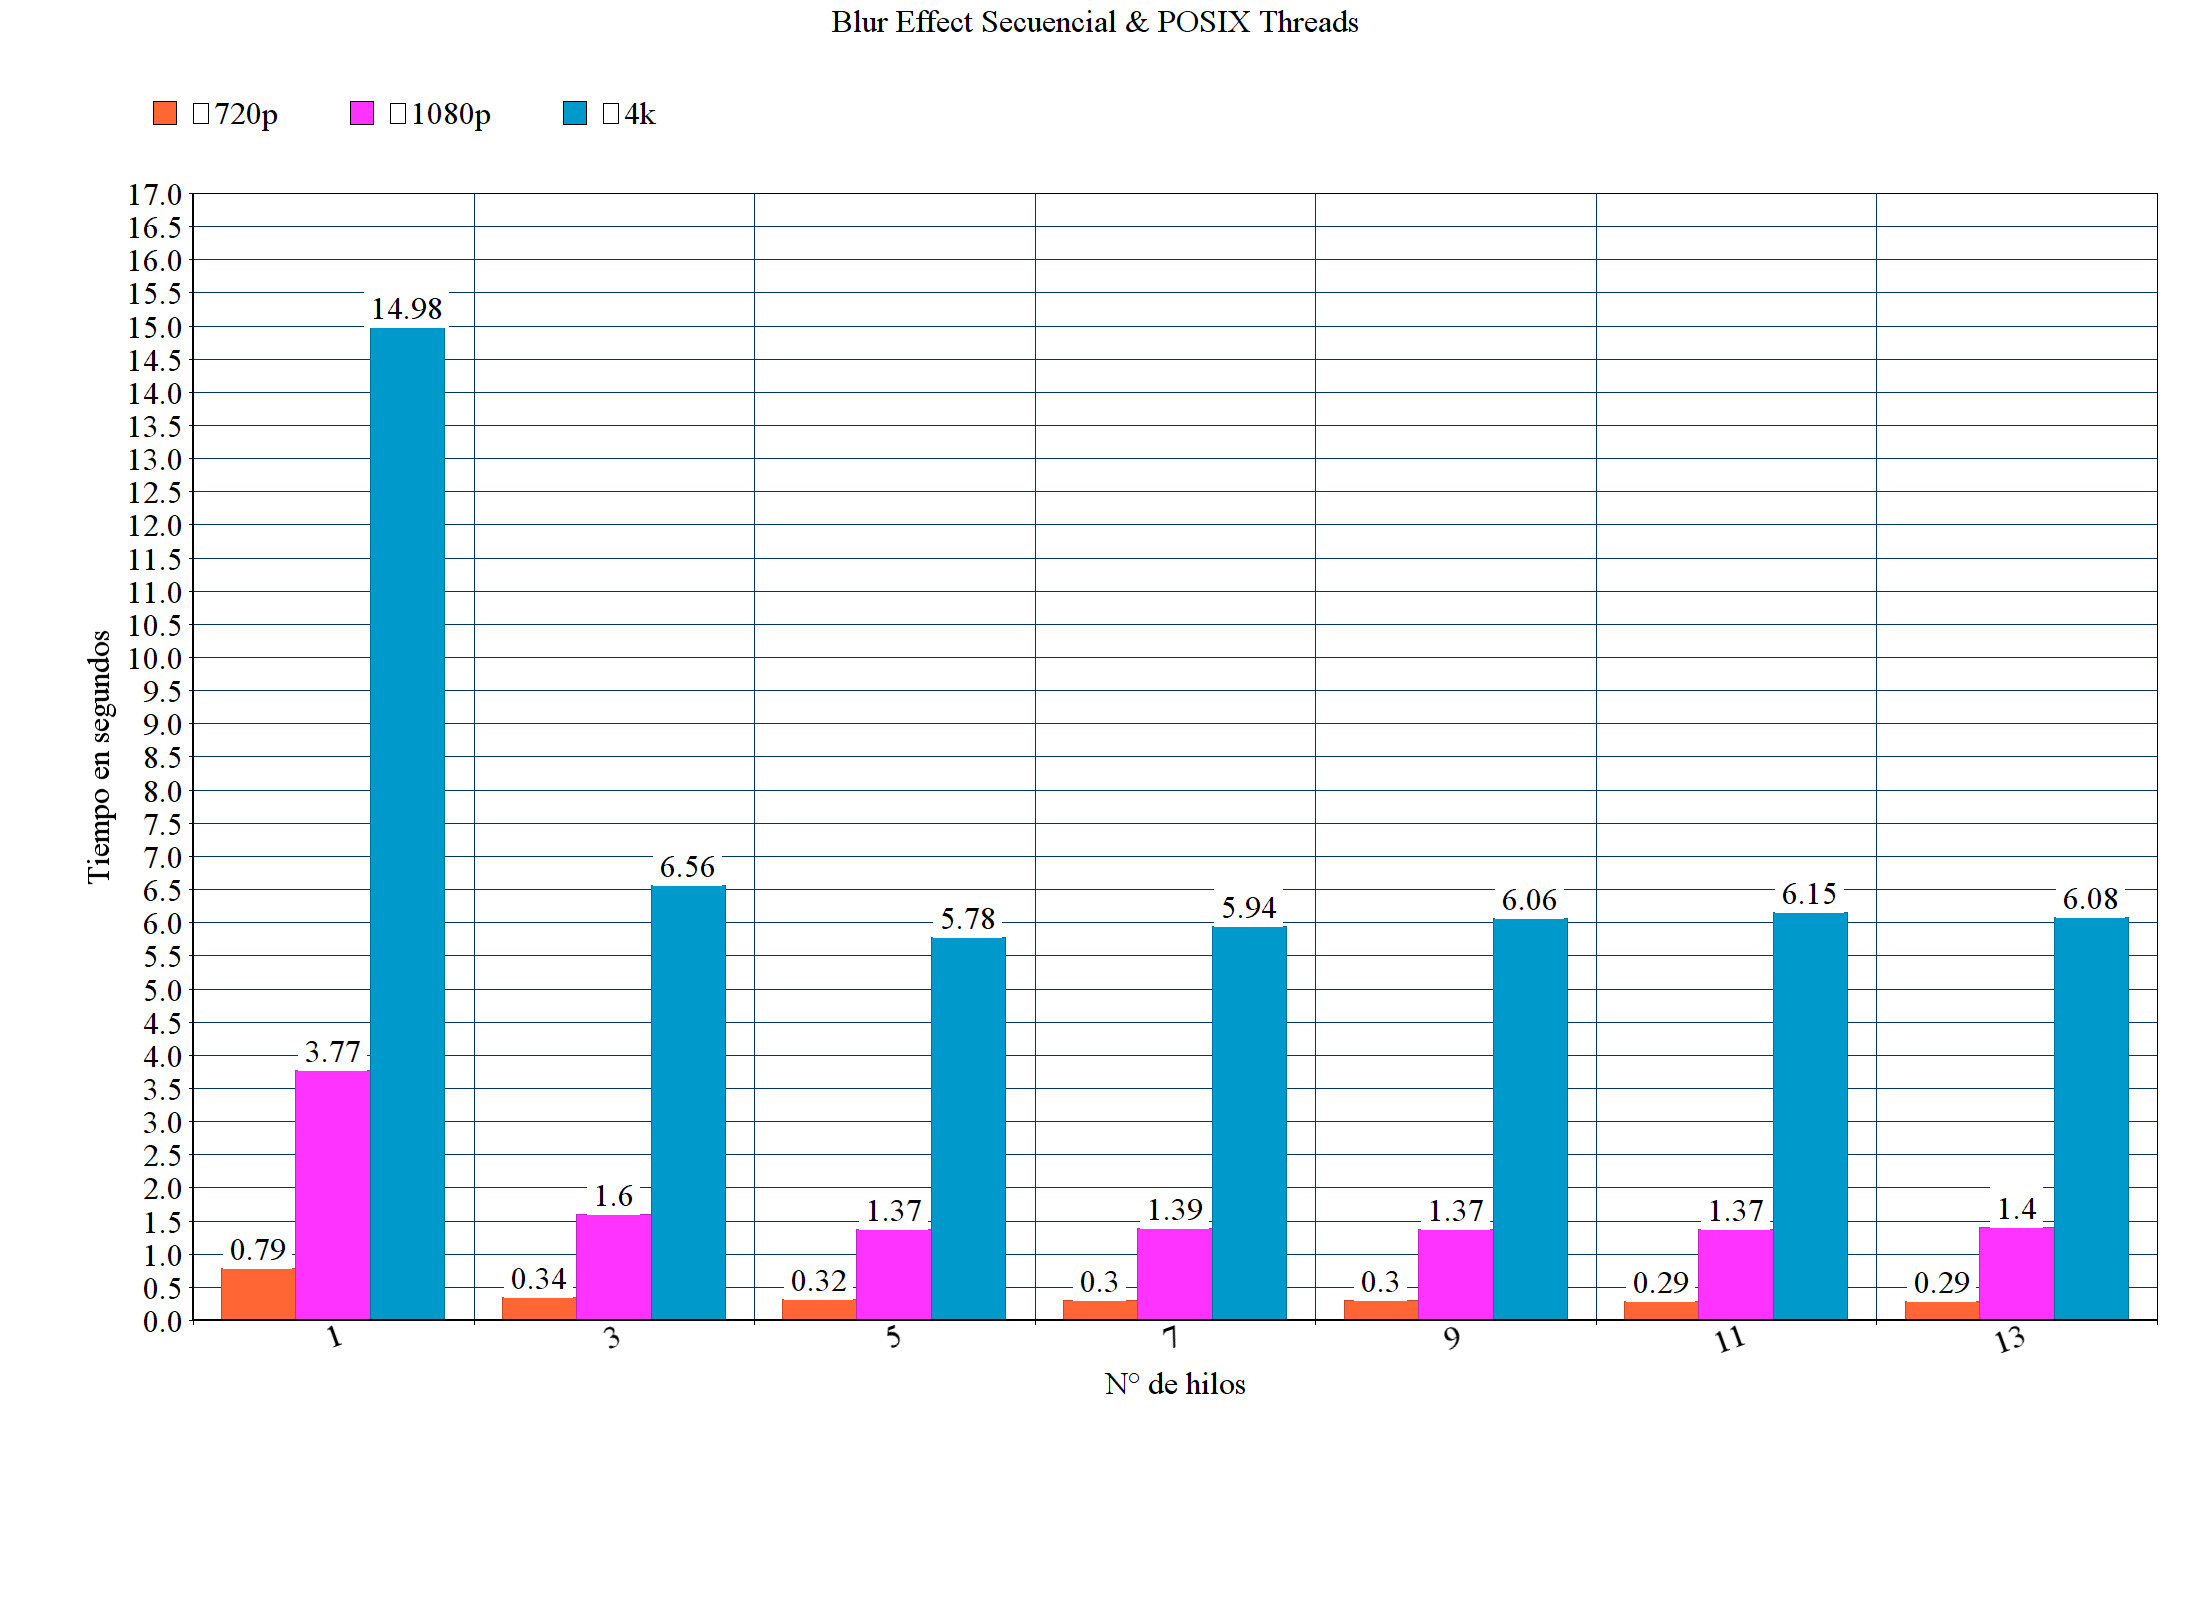
\includegraphics[width=0.42\textwidth]{graph1}
\caption{Variación con POSIX Threads} \label{fig:fig2}
\end{figure}
Con respecto a su forma secuencial, es decir, con un solo hilo se muestra como varían abruptamente las relaciones de tiempo de ejecución del algoritmo respecto al número de hilos que usan para hacer el efecto de blur, se notó en el proceso "anomalias" respecto al tiempo que se demora en ejecutar el algoritmo despues de determinado número de hilos, observe la tabla 1
\begin{table}[H]
\centering
\begin{tabular}{|p{1.5cm}||p{1.5cm}|p{1.5cm}|p{1.5cm}| }
\hline 
•&	720p&	1080p&	4k \\
\hline 
\hline 
1&	0.58&	1.28&	8.38\\
3&	0.44&	0.88&	4.99\\
5&	0.42&	0.82&	4.83\\
7&	0.41&	0.77&	4.77\\
9&	0.38&	0.77&	4.73\\
11&	0.37&	0.75&	4.73\\
13&	0.36&	0.72&	4.72\\
\hline		
\end{tabular} 
\caption{Tiempos con OMP} \label{table:table2}
\end{table}
\begin{figure}[H]
\centering
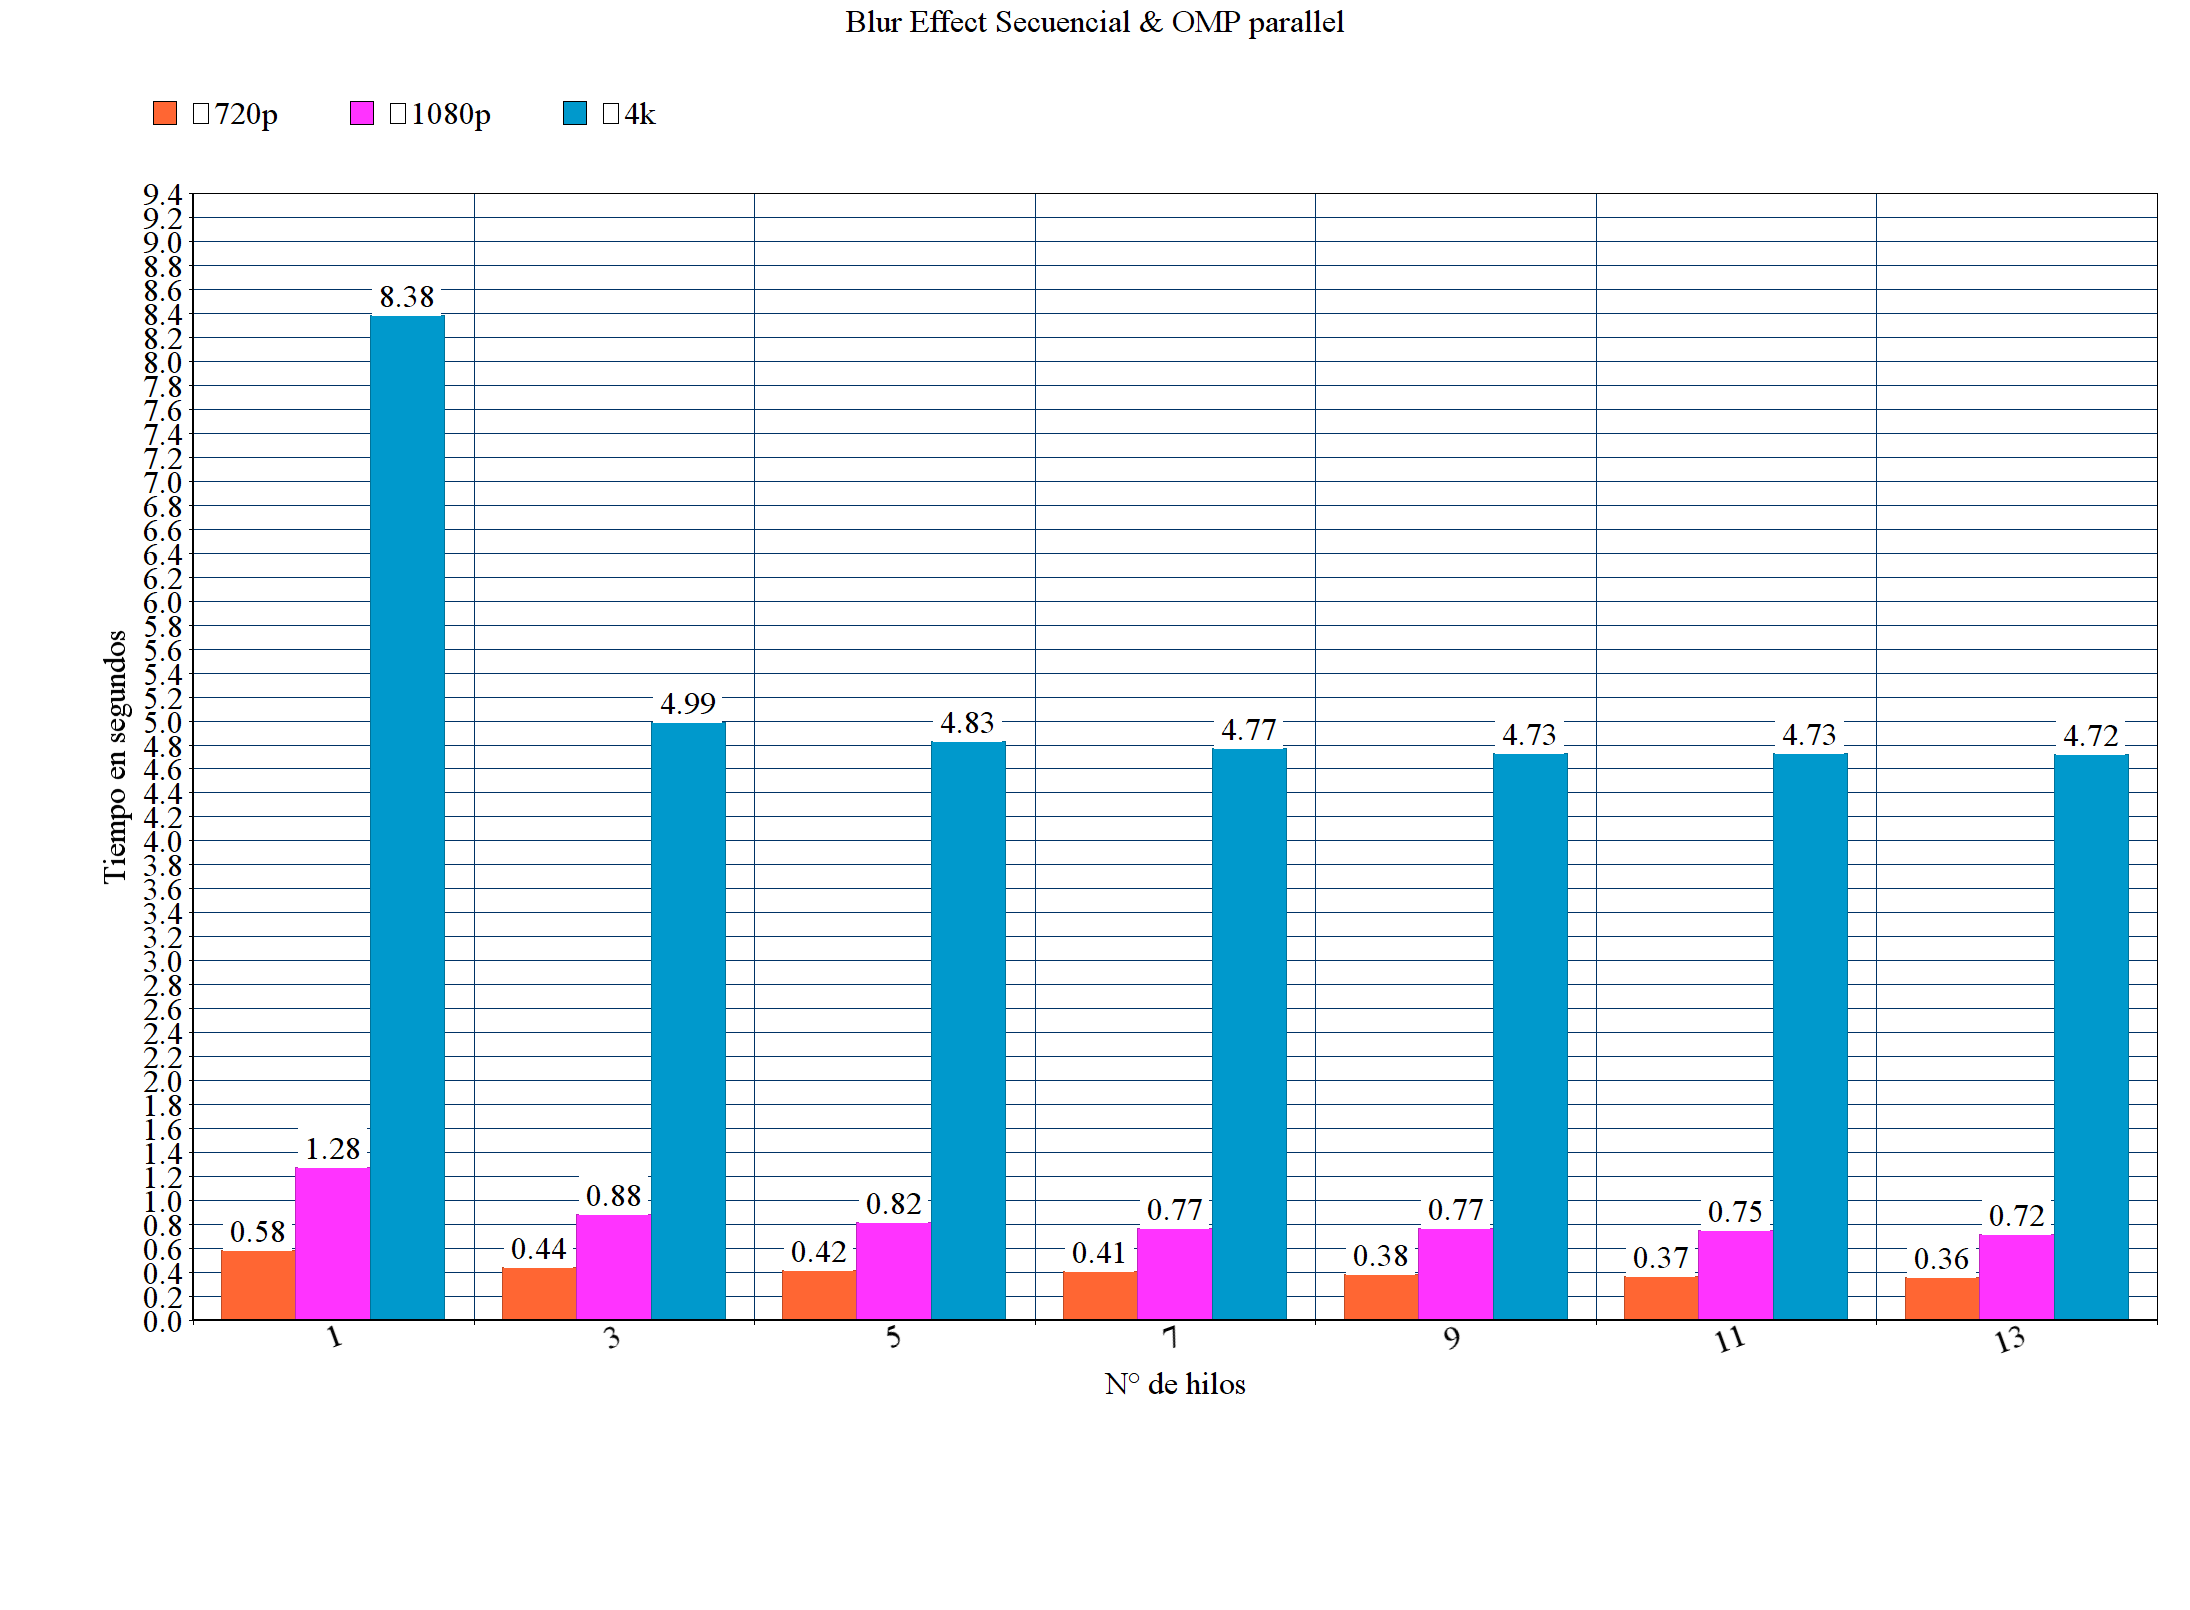
\includegraphics[width=0.42\textwidth]{graph2}
\caption{Variación con OMP} \label{fig:fig3}
\end{figure}
\end{enumerate}

Lo mismo sucede en el uso de OMP, en tanto aumentan el número de hilos parece disminuir considerablemente el tiempo de ejecución del algoritmom en esta ocasión el tiempo se mantiene más o menos constante despues de cierto número de hilos, observe la tabla2, y no aumenta.


\begin{table}[H]
\centering
\begin{tabular}{|p{1.5cm}||p{1.5cm}|p{1.5cm}|p{1.5cm}| }
\hline 
•&	720p&	1080p&	4k \\
\hline 
\hline 
16 	&	0.45	&	0.46	& 	0.62	\\
32 	&	0.43	&	0.47	&	0.61	\\
64 	&	0.43	&	0.48	& 	0.60	\\
128 &	0.42	&	0.48	&	0.58	\\
256 &	0.43	&	0.48	&	0.61	\\
512	&	0.45	&	0.48	&	0.63	\\
\hline		
\end{tabular} 
\caption{Tiempos con CUDA} \label{table:table3}
\end{table}
\begin{figure}[H]
\centering
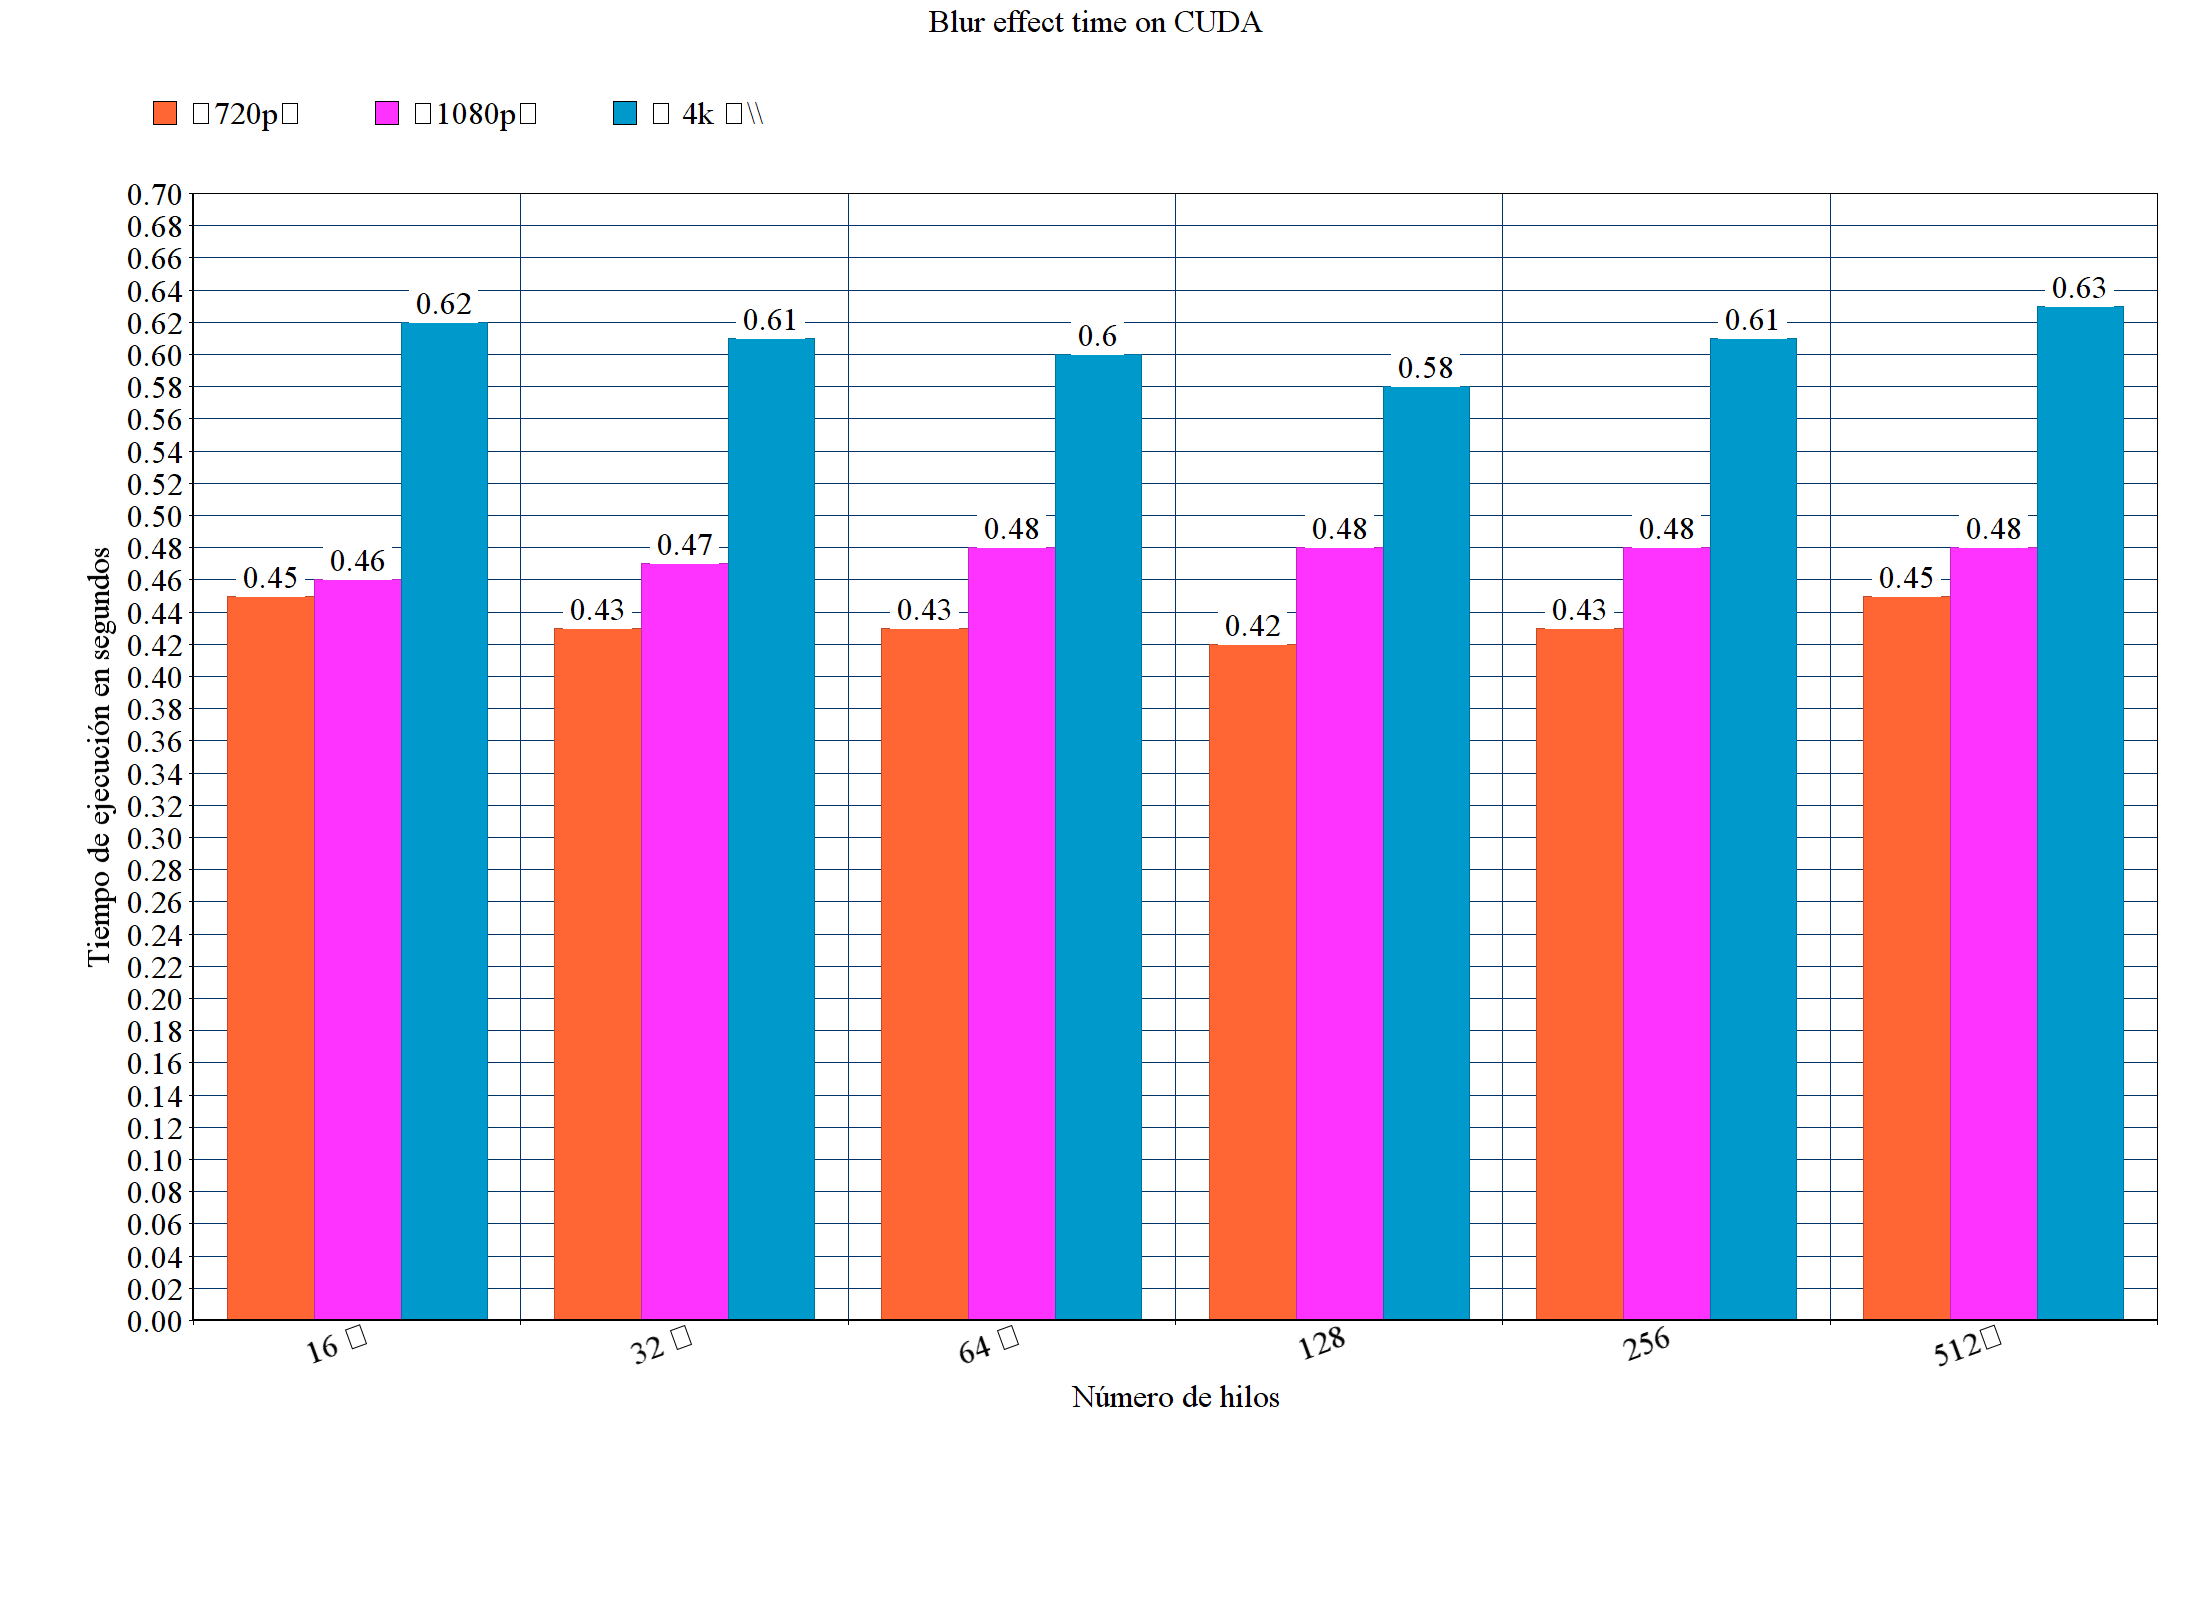
\includegraphics[width=0.42\textwidth]{graph3}
\caption{Variación con CUDA} \label{fig:fig4}
\end{figure}


A diferencia de los experimentos anteriores en esta ocasión se realizó la parelización usando CUDA, perteneciente a las herramientas de la GPU de NVIDIA, se observó un cambio sustacial respecto a la parelización en la CPU, la paralelización de nuestro algoritmo en GPU se realizó con una candidad mucho mayor de hilos y se obtuvo cierta estabilidad a diferencia de los otros casos (POSIX y OMP)


\section*{Conclusiones.}

Se logró mostrar que la paralelización es una herramienta que permite a desarrolladores en distintos campos optimizar el tiempo de ejecución y consumo de recursos esto, en el caso concreto del algoritmo Gaussian Blur Effect fue demostrado con creces, ya que se notó un drastico cambio en los tiempos respecto el número de hilos iba aumentando.

Además se logró mostrar que existen herramientas que pueden hacer más o menos complicada la paralelización de procesos, tareas, en nuestro caso exploramos dos de las más populares, estas POSIX Threads y Open MP que nos permitieron mostrar que si bien el acceso directo y tener un mayor control sobre los hilos, su creación y forma de ejecución es una ventaja que brinda una API de bajo nivel como PThread, por lo menos en tiempos de ejecución, incluso, con el mismo número de hilos, no se compara con herramientas como Open MP.

\noindent 
\bibliographystyle{unsrt}

\bibliography{paralela1}
http://blog.ivank.net/fastest-gaussian-blur.html
OpenCV User Site: http://opencv.org/

\end{document}